% figures/clinic-case.tex
\documentclass[11pt]{article}
\usepackage[margin=1.5cm]{geometry}
\usepackage{tikz}
\usetikzlibrary{positioning,shapes.geometric,arrows.meta,calc}
\pagestyle{empty}
\begin{document}
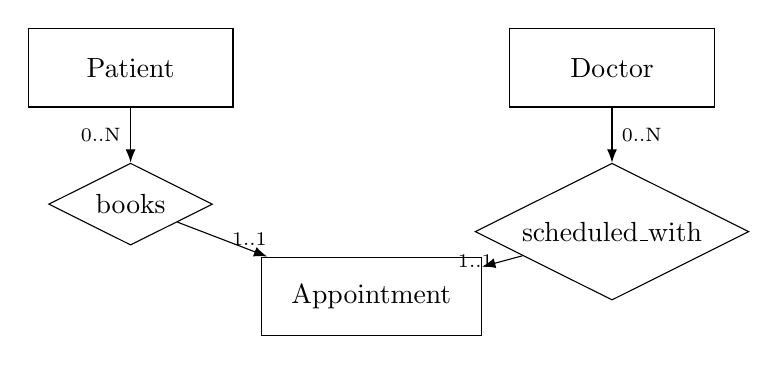
\begin{tikzpicture}[node distance=18mm, >=Latex]
  \node[draw, rectangle, minimum width=2.6cm, minimum height=1cm] (Patient) {Patient};
  \node[draw, rectangle, minimum width=2.6cm, minimum height=1cm, right=35mm of Patient] (Doctor) {Doctor};
  \node[draw, rectangle, minimum width=2.8cm, minimum height=1cm, below=24mm of $(Patient)!0.5!(Doctor)$] (Appt) {Appointment};

  \node[draw, diamond, aspect=2, minimum width=1.6cm, minimum height=1cm, below=7mm of Patient] (Books) {books};
  \node[draw, diamond, aspect=2, minimum width=1.6cm, minimum height=1cm, below=7mm of Doctor] (Sched) {scheduled\_with};

  \draw[->] (Patient) -- (Books) node[midway, left, font=\scriptsize] {0..N};
  \draw[->] (Books) -- (Appt) node[midway, right, font=\scriptsize] {1..1};

  \draw[->] (Doctor) -- (Sched) node[midway, right, font=\scriptsize] {0..N};
  \draw[->] (Sched) -- (Appt) node[midway, left, font=\scriptsize] {1..1};
\end{tikzpicture}
\end{document}
